\documentclass[_main.tex]{subfiles}
 
\begin{document}

%%%%%%%%%%%%%%%%
\part*{Methods}
\label{supp_methods}

\section{A framework for modelling the coalescent process}

\subsection{The coalescent process when \texorpdfstring{$\chi = 0$}{chi is zero}}
\label{supp_coal_chi_zero}

To understand the coalescent properties of the genomic transmission graph, it is instructive to start by considering a parasite population with no superinfection, i.e. $\chi =0$.

Imagine that we sample two alleles from different hosts and, focusing on a point locus, we follow their lineages back in time until they coalesce in a common ancestral allele, as illustrated in figure \ref{fig:coalescent}.  Let \textbf{T} be a random variable representing time to coalescence of the two alleles.

If we sample two alleles from different hosts in the same generation, they are by definition on \textit{separate} transmission chains, but if we trace their lineages back in time they will eventually \textit{meet} in the same host and thus in the same transmission chain.  If two lineages are separated in generation $t$ then the probability that they meet in generation $t-1$ is $1/N_h$.   Let $T_1$ be the expectation of the time taken for two lineages to meet in the same host.

\begin{equation*}
T_1 = 
\sum_{i=1}^\infty
i \Big( \frac{1}{N_h} \Big)
\Big( 1 - \frac{1}{N_h} \Big)^{i-1}
 = N_h
\end{equation*}

Once the two lineages have met in the same host, as we proceed back in time, the two lineages are \textit{cotransmitted} along the same transmission chain until they eventually \textit{coalesce} in a common ancestral allele.  If two lineages are cotransmitted in generation $t$ then the probability that they coalesce in generation $t-1$ is $1/Q$.  Let $T_2$ be the expectation of the time taken for two lineages to coalesce after meeting in the same transmission chain.

\begin{equation*}
T_2 =
\sum_{j=0}^\infty
j \Big( \frac{1}{Q} \Big)
\Big( 1 - \frac{1}{Q} \Big)^{j}
= Q - 1
\end{equation*}

Here we are allowing for the possibility that coalescence could occur as soon as two lineages meet in the same host, as represented by the condition $j=0$ in the above expression.   We can now combine these two parts to get the expectation of time to coalescence:

\begin{equation*}
E \{ \textbf{T} \}   
= T_1 + T_2
= N_h + Q - 1
\end{equation*}

%%%%%%%%%%%%%%%%
\subsection{The coalescent process when \texorpdfstring{$\chi \ge 0$}{chi >= 0}}
\label{supp_coalescent}
%%%%%%%%%%%%%%%%

Imagine that we sample two alleles at some point locus and follow the two lineages back in time until they coalesce, as illustrated in figure \ref{fig:graph_1}.  At any point in time the system must be in one of three states:

\begin{itemize} [noitemsep]

\item \textsc{separated} - the two lineages are in different hosts

\item \textsc{cotransmitted} - the two lineages are in the same host

\item \textsc{coalesced} - the two lineages have coalesced

\end{itemize}

\noindent If two lineages are separated and we go back a single generation, these are the possibilities:

\begin{enumerate}

\item the two lineages meet in the same host ($\Pr = 1/N_h$) and

\begin{enumerate}

\item they coalesce ($\Pr = 1/Q$) 

\item they are cotransmitted ($\Pr = 1 - 1/Q$) 

\end{enumerate}

\item or the two lineages stay separated ($\Pr = 1 -  1/N_h$)

\end{enumerate}

from which we obtain these transition probabilities:

\begin{equation*} \label{eq:supp_coal1}
\Pr \{ \textsc{\small{separated}} \rightarrow \textsc{\small{separated}} \} 
= 1 - \frac{1}{N_h}
\end{equation*}

\begin{equation*} \label{eq:supp_coal2}
\Pr \{ \textsc{\small{separated}} \rightarrow \textsc{\small{cotransmiitted}} \} 
= \frac{1}{N_h} (1 - \frac{1}{Q})
\end{equation*}

\begin{equation*} \label{eq:supp_coal3}
\Pr \{ \textsc{\small{separated}} \rightarrow \textsc{\small{coalesced}} \} 
= \frac{1}{N_hQ}
\end{equation*}

\noindent If two lineages are cotransmitted and we go back a single generation, these are the possibilities:

\begin{enumerate}

\item there is one source of infection ($\Pr = 1 -\chi$)

\begin{enumerate}

\item the lineages coalesce ($\Pr = 1/Q$)

\item the lineages remain cotransmitted ($\Pr = 1 - 1/Q$)

\end{enumerate}  

\item there are two sources of infection ($\Pr = \chi$)

\begin{enumerate}

\item the lineages come from different sources ($\Pr = Q/(2Q-1)$)

\item the lineages come from the same source  ($\Pr = (Q-1)/(2Q-1)$)

\begin{enumerate}

\item they coalesce ($\Pr = 1/Q$) 

\item they are cotransmitted ($\Pr = 1 -1/Q$). 

\end{enumerate} 

\end{enumerate}

\end{enumerate} 

from which we obtain these transition probabilities:

\begin{equation*} \label{eq:supp_coal4}
\Pr \{ \textsc{\small{cotransmitted}} \rightarrow \textsc{\small{separated}} \} 
= \frac{Q\chi}{2Q-1}
\end{equation*}

\begin{equation*} \label{eq:supp_coal5}
\Pr \{ \textsc{\small{cotransmitted}} \rightarrow \textsc{\small{cotransmitted}} \} 
= \frac{(Q-1)(2Q - Q\chi - 1)}{Q(2Q-1)}
\end{equation*}

\begin{equation*} \label{eq:supp_coal6}
\Pr \{ \textsc{\small{cotransmitted}} \rightarrow \textsc{\small{coalesce}} \} 
= \frac{2Q - Q\chi - 1}{Q(2Q-1)}
\end{equation*}

Based on these observations we can construct a matrix of transition probabilities for the three possible states of two lineages as we proceed back in time through the transmission graph (table \ref{tab:main_tr_matrix}).

\subsection{Markov chain simulation of time to coalescence} 
\label{supp_mcs}

Using the matrix of transmission probabilities (table \ref{tab:main_tr_matrix}) we can calculate the probability distribution of time to coalescence for any combination of the transmission parameters $N_h$, $Q$ and $\chi$.  As we have seen, if we follow two lineages back in time they can be in three possible states: (a) separated or (b) cotransmitted or (c) coalesced.  Let $P_{a,t}$, $P_{b,t}$ and $P_{c,t}$ respectively denote the probabilities of these states at time $t$.  We can represent the overall state of the system at time $t$ by a probability vector $\textbf{X}_t$ where

\begin{equation*} 
\textbf{X}_t =
\begin{bmatrix}
P_{a,t} & P_{b,t} & P_{c,t}
\end{bmatrix}
\end{equation*}

Let $\textbf{Y}$ be a matrix of transition probabilities, where $y_{ij}$ is the probability that state $i$ will transition to state $j$ if we go back a single generation, as represented in table \ref{tab:main_tr_matrix}.  As we move back in time, i.e. as we proceed from time $t$ to $t-1$,

 \begin{equation*} 
\textbf{X}_{t-1} =
\textbf{X}_{t} \textbf{Y}
\label{eq:supp_markov}
\end{equation*}

This allows us to compute the probability of each state at any given time by Markov chain simulation.  In each simulation, we sample two imaginary alleles and follow their lineages back in time, recalculating the probability of each state as we move from generation to generation, as shown in figure \ref{fig:main_markov_4}.

To study between-host variation we specify that two alleles are sampled from different hosts, i.e. at the start of the simulation $\textbf{X}_0 = \begin{bmatrix} 1 & 0 & 0 \end{bmatrix}$.  Alternatively, we can study within-host variation by specifying that two alleles are sampled from the same host, i.e. $\textbf{X}_0 = \begin{bmatrix} 0 & 1 & 0 \end{bmatrix}$.   By running the Markov chain simulation over many generations we obtain the probability distribution of coalescence time, as illustrated in figure \ref{fig:main_markov_3}.   

%%%%%%%%%%%%

\subsection{Coalescence time when \texorpdfstring{$\chi =1$ and $Q =1$}{chi=1 and Q=1}}
\label{supp_anomaly}

In general, two alleles sampled from the same host coalesce more rapidly than two alleles sampled from different hosts.   This difference is marked when $\chi=0$.  As $\chi$ increases, the coalescence time of two alleles sampled from the same host starts to approach that of two alleles sampled from different hosts, and when $\chi=1$ the difference becomes relatively small.  

There is an exception to this general rule.  When $\chi=1$ and $Q=1$, the mean coalescence time of two alleles sampled from the same host is exactly one generation greater than that of two alleles sampled from different hosts.  This apparent anomaly arises because, in this situation, the two alleles acquired by a host must come from different source hosts so they cannot coalesce in the generation prior to that in which they are sampled.

%%%%%%%%%%%%

\section{Genetic variation at a point locus}
\label{supp_point_locus}

Imagine that we sample two alleles at a point locus and trace their lineages back in time until they coalesce.  The two alleles must have the same DNA sequence if neither lineage is affected by mutation.  In principle the two alleles could have the same DNA sequence if both lineages are affected by mutation but we rule out this possibility by assuming an `infinite alleles' model.  Let $u$ be the mutation rate per generation at this locus, let $G$ be the homozygosity of the locus, and let \textbf{T} be a random variable representing the time to coalescence of two lineages measured in generations.

\begin{equation*}
G = (1 - u)^{2 \textbf{T}}
\label{eq:supp_G}
\end{equation*}

Let $H$ be the heterozygosity of our point locus, where $H = 1 - G$.  We obtain the expectation of $H$ for any two alleles sampled at random from the population by summing over the probability distribution of time to coalescence.  
  
\begin{equation*}
E \{ H  \} = 1 - \sum_{i=1}^\infty \Pr \{ \textbf{T} = i \} \times (1-u)^{2i}
\end{equation*}

Let $T_C$ be the mean time to coalescence measured in generations.  If $u$ is sufficiently small (say $<10^{-5}$) we can safely ignore factors of $u^2$ and above to make the approximation

\begin{equation*}
E \{ H  \} \approx 1 - \sum_{i=1}^\infty \Pr \{ \textbf{T} = i \}  + 2u \sum_{i=1}^\infty i\Pr \{ \textbf{T} = i \}
\end{equation*}

\begin{equation*}
E \{ H \} \approx 2 u T_C
\label{eq:supp_het_approx}
\end{equation*}

%%%%%%%%%%%%%%%%%%

\subsection{Nucleotide diversity of the global parasite population}
\label{supp_global_pi}

The MalariaGEN Pf6 and Pf7 datasets \cite{MalariaGEN2021,MalariaGEN2023} both contain estimates of $\pi$ based on coding regions of the core \textit{P. falciparum} genome.  The results differ between the two datasets as can be seen by comparing the upper and lower panels of figure \ref{fig:Pf6_global_pi}.  In African samples, the median value of $\pi$ is $\sim 2.5 \times 10^{-4}$ in Pf6 and $\sim 5 \times 10^{-4} $ in Pf7.  This difference could be partly because the Pf6 estimate is restricted to biallelic SNPs whereas the Pf7 estimate includes multiallelic SNPs.  Another factor is that Pf7 has approximately twice as many high-quality SNPs and short indels as Pf6 (6 versus 3 million), probably due to a combination of increased sample size and minor alterations to the variant calling algorithms.

\begin{figure}[h!]
\centering
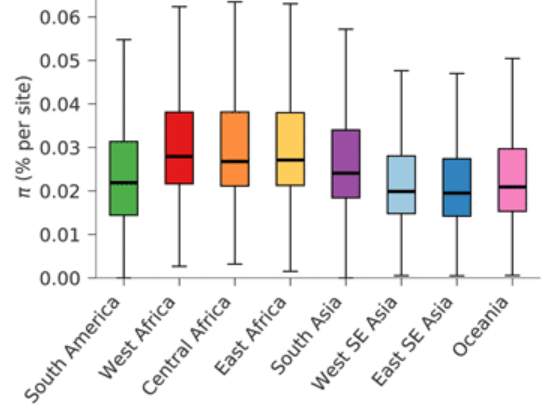
\includegraphics[width=7cm]{230217_Pf6_global_pi.png}
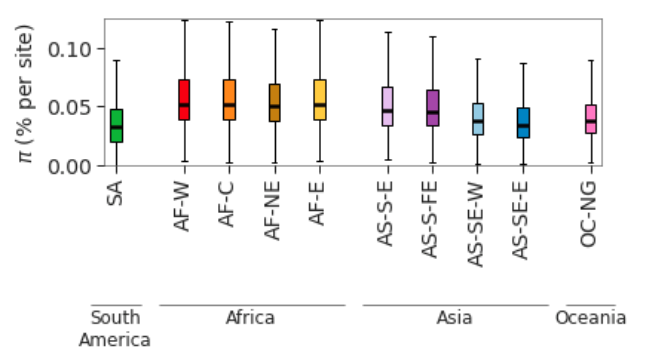
\includegraphics[width=10cm]{230217_Pf7_global_pi.png}
\caption{\textbf{Estimates of nucleotide diversity in coding regions of the \textit{P. falciparum} genome.}  Upper panel is copied from the MalariaGEN Pf6 dataset (reference \cite{MalariaGEN2021} fig. 2) and lower panel is from the MalariaGEN Pf7 dataset (reference \cite{MalariaGEN2023} supp. fig. 6).   Thick lines represent median values, boxes show the interquartile range, and whiskers represent the bulk of the distribution, discounting outliers.  Possible reasons for differences between the Pf6 and Pf7 results are discussed in the text.  
}
\label{fig:Pf6_global_pi}
\end{figure}

The reason for considering only coding regions is that non-coding regions are error-prone for variant calling due to their very high AT content with many short tandem repeats.  Our algorithms are attuned to minimise variant calling errors but both false positive and false negative results are possible. Note also that some \textit{P. falciparum} genes are under purifying selection (which tends to reduce $\pi$) while others are under diversifying selection (which tends to increase $\pi$).  

In this paper we use $\pi \approx 4 \times 10^{-4}$ as a first approximation for the global parasite population, but it will be clear that there are multiple potential sources of error and this could be either an overestimate or an underestimate. 

%%%%%%%%%%%%%

\section{Genetic variation at a haplotype locus}

\subsection{Shared haplotype segments}
\label{supp_shs}

Shared haplotype segments are segments of the genome where two parasites have identical DNA sequences.   Unrelated parasites often have some shared haplotype segments that extend over a few kilobases, but if we observe a substantial number of shared haplotype segments that are hundreds of kilobases long, this suggests that the parasites share a recent common ancestor.  

We would like to evaluate the expected proportion of the genome that is occupied by shared haplotype segments.  Imagine a chromosome of length $c$ centimorgans that is divided into non-overlapping blocks of one centimorgan size as illustrated in figure \ref{fig:haplotype_blocks}.  We are interested in shared haplotype segments of $> 2$ centimorgans and so we will make the simplifying assumption that haplotype loci are constructed of an integral number of these one centimorgan blocks.  More precisely, we specify that a haplotype locus that occupies $i$ blocks of the imaginary chromosome has a real length in the interval $(i-1, i]$ centimorgans.  

\begin{figure}[h!]
\centering
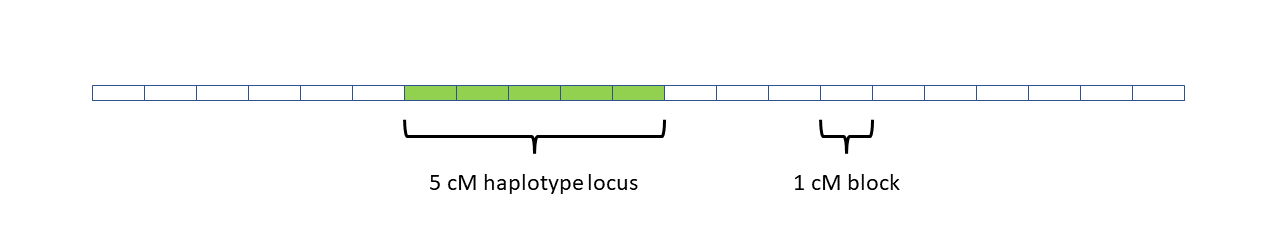
\includegraphics[width=15cm]{230228_haplotype_blocks.png}
\caption{\textbf{Simplified architecture of a haplotype locus.}  We imagine that a chromosome is divided into non-overlapping blocks of 1 centimorgan size, and that each haplotype locus is constructed of an integral number of these blocks.  Thus a haplotype locus in the interval $(4, 5]$ centimorgans is considered to be 5 blocks.  
}
\label{fig:haplotype_blocks}
\end{figure}

Take a haplotype locus of $i$ blocks and let $g_i$ be the probability that this is a shared haplotype segment with respect to two alleles randomly sampled from the population.  We can evaluate $g_i$ from equation \ref{eq:main_G_L_mean} since:

\begin{equation*}
g_i = E \{G_{i -1} \} - E \{G_{i} \}
\end{equation*}

Let $\omega_i$ be the expected number of shared haplotype segments of $i$ blocks.  The number of $i$-block segments that can be fitted into a chromosome is $c/i$, so we will make the very crude approximation that  

\begin{equation*}
\omega_i \approx g_i \times \frac{c}{i}
\end{equation*}

To quantify identity by descent (IBD) we are interested in shared haplotype segments of above a certain size.  The total length of shared haplotype segments of $>k$ centimorgans is given by the sum

\begin{equation*}
\sum_{i = k + 1}^c i \omega_i \approx \sum_{i = k +1 }^c \frac{i g_i c}{i} \approx \sum_{i = k +1 }^c g_i c
\end{equation*}

Thus the proportion of the chromosome occupied by shared haplotype segments of $>k$ centimorgans is very approximately given by

\begin{equation}
\sum_{i = k + 1}^c i \omega_i \div c
= \sum_{i = k +1 }^c g_i 
= E \{G_k \}
\end{equation}

We can extrapolate this result to the whole genome.   This tells us that the proportion of the genome occupied by shared haplotype segments of $>2$ centimorgans can be crudely approximated by $\gamma$, the mean haplotype homozygosity of a 2 centimorgan locus (figure \ref{fig:main_hap_hom_27}).   

%%%%%%%%%%%%%%%%%%%%%%

\section{Migration in a hierarchical population structure}

\label{supp_migration_1}

Imagine that we sample two alleles from a local subpopulation of parasites that is embedded within a much larger metapopulation, and follow the two lineages back in time until they coalesce.  

If we sample two alleles from the subpopulation and go back in time, the two lineages have six possible states: (i) in different hosts in the subpopulation; (ii) in the same host in the subpopulation; (iii) in different hosts in the metapopulation; (iv) in the same host in the metapopulation; (v) one lineage in the subpopulation and the other in the metapopulation; (vi) coalesced.  We could work out the transition probabilities between these six states, but if the metapopulation is much larger than the subpopulation then we can make some simplifying assumptions that will help to clarify the population dynamics as well as speeding up our Markov chain simulations.

Let $m$ be the probability that a host within the local subpopulation acquired their infection from the metapopulation, and let the number of such hosts per generation be $N_m = m N_h$.  These migrant hosts could be either immigrants from the metapopulation or local residents who have been travelling outside the local area.  Let $m'$ be the probability that a host within the metapopulation acquired their infection from the local parasite subpopulation, and let $N'_m$ and $N'_h$ be corresponding terms for the metapopulation.  

Coalescence must occur either in the subpopulation or the metapopulation.  If the metapopulation is much larger than the local subpopulation ($N_h' \gg N_h$) and if absolute rates of migration between the two populations are approximately symmetrical ($m' N_h' \approx m N_h$) then it must be the case that $m' \ll m$.   Thus if one lineage moves from the subpopulation into the metapopulation (as we proceed back in time) then it is very unlikely that it will move back into the subpopulation before the other lineage joins it in the metapopulation.  In other words, as soon as one lineage has entered the metapopulation, then it becomes highly probable that coalescence will eventually occur in the metapopulation.  

Thus we can consider the metapopulation as an absorbing state from the perspective of the subpopulation, because once a lineage has entered the metapopulation we might as well treat both lineages as being in the metapopulation, as that is where they must coalesce. This allows us to organise our simulation into two compartments:   

\begin{enumerate}

\item When we model the behaviour of two lineages within the subpopulation, there are four possible states:

\begin{enumerate}

\item in different hosts in the subpopulation

\item in the same host in the subpopulation

\item coalesced in the subpopulation (absorbing state)

\item entered the metapopulation (absorbing state)

\end{enumerate}

\item If a lineage goes into the metapopulation, we treat both lineages as being in the metapopulation and consider three possible states:

\begin{enumerate}

\item in different hosts in the metapopulation

\item in the same host in the metapopulation

\item coalesced within the metapopulation (absorbing state)

\end{enumerate}

\end{enumerate}

Framed in this way, the metapopulation is equivalent to the simple population whose transition probability matrix is given by table \ref{tab:main_tr_matrix}.   The transition probabilities of the subpopulation can be worked out as follows.  

%%%%%%%%%%%%%%%%%%%

\paragraph{If two lineages are separated within the subpopulation} and we go back a generation, these are the possible outcomes:

\label{supp_trans_matrix_2}

\begin{enumerate} [noitemsep]

\item They are in the same host.  $\Pr = 1/N_h$

\begin{enumerate} [noitemsep]

\item They coalesce. $\Pr = 1/Q$

\item They are cotransmitted. $\Pr = 1 - 1/Q$

\begin{enumerate} [noitemsep]

\item They remain in the subpopulation. $\Pr = 1 - m$ 

\item They enter the metapopulation. $\Pr = m$

\end{enumerate}

\end{enumerate}

\item They are not in the same host. $\Pr = 1 - 1/N_h$

\begin{enumerate} [noitemsep]

\item Both remain in the subpopulation. $\Pr = (1 - m)^2$

\item One or both enter metapopulation. $\Pr = 2m - m^2$

\end{enumerate}

\end{enumerate}

\noindent From this we obtain

\begin{equation*}
\Pr \{ \textsc{\small{separated}} \rightarrow \textsc{\small{coalesced}} \} 
= \frac{1}{N_h Q}
\end{equation*}

\begin{equation*}
\Pr \{ \textsc{\small{separated}} \rightarrow \textsc{\small{cotransmitted}} \} 
= \frac{(Q -1)(1-m)}{N_h Q}
\end{equation*}

\begin{equation*}
\Pr \{ \textsc{\small{separated}} \rightarrow \textsc{\small{separated}} \} 
= \frac{(N_h - 1)(1-m)^2}{N_h}
\end{equation*}

\begin{equation*}
\Pr \{ \textsc{\small{separated}} \rightarrow \textsc{\small{metapopulation}} \} 
= \frac{(Q -1)m}{N_h Q} + \frac{(N_h-1)(2m - m^2)}{N_h}
\end{equation*}

\begin{equation*}
= \frac{m(Q-1) + Q (N_h-1)(2m - m^2)}{N_h Q}
\end{equation*}

%%%%%%%%%%%%%%%%%%

\paragraph{If two lineages are cotransmitted within the subpopulation} and we go back a generation, these are the possible outcomes:

\begin{enumerate} [noitemsep]

\item If the current host is multiply infected. $\Pr = \chi$

\begin{enumerate} [noitemsep]

\item They remain cotransmitted.  $\Pr = (Q-1)/(2Q-1)$

\begin{enumerate} [noitemsep]

\item They coalesce. $\Pr = 1/Q$

\item They do not coalesce. ($\Pr = 1 - 1/Q$)

\begin{enumerate} [noitemsep]

\item They remain in the subpopulation. $\Pr = 1 - m$ 

\item They enter the metapopulation. $\Pr = m$

\end{enumerate}

\end{enumerate}

\item They become separated. $\Pr = Q/(2Q-1)$

\begin{enumerate} [noitemsep]

\item They both remain in the subpopulation. $\Pr = (1 - m)^2$ 

\item One or both enters the metapopulation. $\Pr = 2m - m^2$

\end{enumerate}

\end{enumerate}

\item If the current host is not multiply infected. $\Pr = 1 - \chi$

\begin{enumerate} [noitemsep]

\item They coalesce. $\Pr = 1/Q$

\item They do not coalesce, i.e. they remain cotransmitted.  $\Pr = 1 - 1/Q$

\begin{enumerate} [noitemsep]

\item They remain within the subpopulation. $\Pr = 1 - m$

\item They enter the metapopulation. $\Pr = m$

\end{enumerate}

\end{enumerate}

\end{enumerate}

\noindent From this we obtain

\begin{equation*}
\Pr \{ \textsc{\small{cotransmitted}} \rightarrow \textsc{\small{coalesced}} \} 
= \frac{2Q - Q \chi - 1}{Q(2Q-1)} 
\end{equation*}

\begin{equation*}
\Pr \{ \textsc{\small{cotransmitted}} \rightarrow \textsc{\small{cotransmitted}} \} 
= \frac{(Q-1)(1-m)(2Q - \chi Q - 1)}{Q(2Q-1)}
\end{equation*}

\begin{equation*}
\Pr \{ \textsc{\small{cotransmitted}} \rightarrow \textsc{\small{separated}} \} 
= \frac{\chi Q (1-m)^2}{2Q-1}
\end{equation*}

\begin{equation*}
\Pr \{ \textsc{\small{cotransmitted}} \rightarrow \textsc{\small{metapopulation}} \} 
= \frac{mQ(2Q - 3 + \chi + \chi Q - m \chi Q) + m}{Q(2Q-1)} 
\end{equation*}

\noindent This gives us a matrix of transition probabilities as shown in table \ref{tab:tr_matrix_subpopulation}

%%%%%%%%%%%%%%%%%


\renewcommand\theadalign{bc} 

\begin{table}[h!] 
\centering
\large{
\begin{tabular}{l | c c c c } 
\hline \\
\textbf{\small{State}} & 
\small{Separated} & 
\small{Cotransmitted} & 
\small{Coalesced} & 
\small{Metapopulation}\\ [0.5ex] 
\hline \\
\small{Separated} & 
$\frac{(N_h - 1)(1-m)^2}{N_h}$ & 
$\frac{(Q -1)(1-m)}{N_h Q}$ &
$\frac{1}{N_h Q}$ &
$\frac{m(Q-1) + Q (N_h-1)(2m - m^2)}{N_h Q}$ \\ [2ex]
\small{Cotransmitted} &
$\frac{Q \chi (1-m)^2}{2Q-1}$ &
$\frac{(Q-1)(1-m)(2Q - Q \chi - 1)}{Q(2Q-1)}$ &
$\frac{2Q - Q \chi - 1}{Q(2Q-1)}$ &
$\frac{mQ(2Q - 3 + \chi + \chi Q - m \chi Q) + m}{Q(2Q-1)}$  \\ [2ex] 
\small{Coalesced} & 0 & 0 & 1 & 0 \\ [2ex] 
\small{Metapopulation} & 0 & 0 & 0 & 1 \\ [2ex] 
\end{tabular}
}
\caption{\small{\textbf{Transition probabilities for the four possible states of two lineages within a subpopulation}. At any point in time, two lineages must be (1) separated within the subpopulation or (2) cotransmitted within the subpopulation or (3) coalesced within the subpopulation or (4) entered the metapopulation. As discussed in the text, if the metapopulation is much larger than the subpopulation then we can treat it as an absorbing state.  Row $i$ column $j$ of the table gives the probability that lineages in state $i$ will transition to state $j$ if we go back a single generation.}}
\label{tab:tr_matrix_subpopulation}
\end{table}

%%%%%%%%%%%%%%%%%%

\section{Analysis of within-host variation}

%%%%%%%%%%%%%%%%%%
\subsection{Within-host heterozygosity in a population with \texorpdfstring{$\chi=0$}{chi=0}}
\label{supp_whh_chi_0}
%%%%%%%%%%%%%%%%%%

First we consider a population in which there is no superinfection, i.e. $\chi = 0$.  We assume that evolution is neutral, i.e. there is no effect of natural selection.  

Imagine that host A transmits parasites to host B. Let $G_A$ be the probability that two alleles sampled from host A are homozygous, and $H_A$ the probability that they are heterozygous, where $H_A = 1 - G_A$.  Likewise $G_B$ and $H_B$ for host B.  The relationship between $H_A$ and $H_B$ will be determined by the combination of genetic drift and mutation in just the same way as the Wright-Fisher model.   

\begin{figure}[h!]
\centering
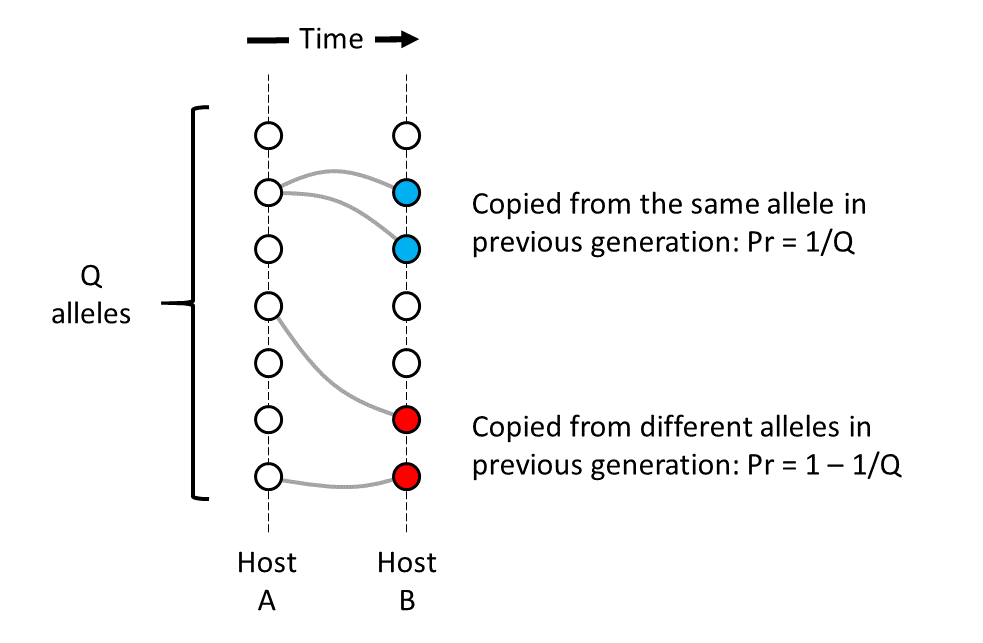
\includegraphics[width=10cm]{181002_isolated_tc_drift.png}
\caption{\textbf{Copying of alleles from one host to the next along a transmission chain with no superinfection.}  Alleles are copied with replacement from $Q$ alleles in the previous generation, exactly analogous to the Wright-Fisher model.}
\label{fig:supp_hahb}
\end{figure}

\paragraph{Genetic drift.}  If we sample two alleles from host B (Figure \ref{fig:supp_hahb}) there are two ways in which they can be homozygous:

\begin{enumerate}[noitemsep]

\item they are copied from the same allele in host A ($ \Pr = 1 / Q $);
\item they are copied from different alleles in host A ($\Pr = 1 - (1/Q) $) but these are homozygous ($\Pr = G_A$).

\end{enumerate}
 
\noindent Since these are mutually exclusive possibilities

\begin{equation}
G_B = \frac{1}{Q} + G_A (1- \frac{1}{Q})
\label{eq:supp_drift}
\end{equation}

\noindent and after substitution and rearrangement

\begin{equation*}
H_B = H_A (1- \frac{1}{Q})
\end{equation*}

\paragraph{Mutation.}  Let $u$ be the probability that an allele is altered by mutation during one generation of transmission.  We assume infinite alleles, i.e. if two alleles are initially homozygous then a mutation in one or both alleles will make them heterozygous.  We can account for mutation by incorporating into equation \ref{eq:supp_drift} the probability of $(1-u)^2$ that neither of the two alleles is affected by mutation:

\begin{equation*}
G_B = \Big( \frac{1}{Q} + G_A (1- \frac{1}{Q}) \Big) (1-u)^2
\label{eq:supp_drift_mut}
\end{equation*}

Since $u$ is generally very small we can usually ignore factors of $u^2$, so after substitution and rearrangement we obtain

\begin{equation}
H_B \approx H_A \Big(1 - \frac{1}{Q} - 2u + \frac{2u}{Q} \Big) + 2u
\label{eq:supp_hahb}
\end{equation}

\paragraph{Hosts that are $x$ generations apart on the same transmission chain.}  Now imagine two hosts that are $x$ generations apart on the same transmission chain.  Let the within-host heterozygosity of the first host (i.e. the one that exists earlier in time) be $H$ and that of the second host be $H'$.  If we apply equation \ref{eq:supp_hahb} over multiple generations we obtain

\begin{equation}
H' \approx H \alpha^x + 2u \sum_{i=0}^{x-1} \alpha^i
\label{eq:supp_alpha_decay}
\end{equation}

where 

\begin{equation}
\alpha = (1 - \frac{1}{Q}) (1 - 2u) 
\label{eq:supp_alpha}
\end{equation}

The first part of equation \ref{eq:supp_alpha_decay} describes geometric decay of the initial heterozygosity due to genetic drift, while the second part describes a new source of heterozygosity that gradually builds up due to the accumulation of mutations, attenuated by drift.  

\paragraph{Equilibrium state of heterozygosity in a non-crossing transmission chain.} If a transmission chain continues for many generations without crossing with another transmission chain, its within host heterozygosity $H_W$ equilibrates when the effect of genetic drift is equal and opposite to the effect of mutation.  We can evaluate this equilibrium value theoretically by letting $x \rightarrow \infty$ in equation \ref{eq:supp_alpha_decay}.  

\begin{equation*}
H_W \approx H \alpha^\infty + 2u \sum_{i=0}^{\infty} \alpha^i
\end{equation*}

\begin{equation*}
= \frac{2u}{1 - 1 + 1/Q + 2u - 2u/Q}
\end{equation*}

\begin{equation}
H_W \approx \frac{2uQ}{1 + 2uQ - 2u}
\label{eq:supp_Hew}
\end{equation}

If we replace $u$ with $\mu$, the genome-wide single nucleotide substitution rate we can obtain $\pi_W$, the expected level of within-host nucleotide diversity in a population where there has been no superinfection for many generations:

\begin{equation*}
\pi_W \approx \frac{2 \mu Q}{1 + 2 \mu Q - 2 \mu}
\end{equation*}

and by rearrangement

\begin{equation*}
Q \approx \frac{\pi_W (1-2\mu)}{2 \mu (1 - \pi_W)} \approx \frac{\pi_W}{2 \mu}
\end{equation*}

%%%%%%%%%%%%%%%%%%%%%%%%%%%%

\subsection{Estimating within-host nucleotide diversity \texorpdfstring{$\pi_W$}{pi-w} from genome sequencing data.}
\label{supp_Q_pi}

To examine the frequency distribution of within-host nucleotide diversity $\pi_W$ in the \href{https://www.malariagen.net/resource/26}{MalariaGEN Pf6 dataset}, we begin by selecting high-quality samples (n = 5,970) and high-quality biallelic coding SNPs with vqslod > 3 (n = 502,221).   We then calculate

\begin{itemize}[noitemsep]

\item within-host heterozygosity for each SNP in each sample

\item mean within-host heterozygosity for each SNP across all samples ($\widehat{H}_W$)

\item mean within-host heterozygosity for each sample across all SNPs ($\widehat{H}_{sample}$)

\end{itemize}

As in section \ref{supp_global_pi}, we restrict our analysis to coding regions because non-coding regions are error-prone due to their very high AT content with many short tandem repeats.  The MalariaGEN Pf6 dataset has quality control processes that endeavour to minimise variant calling errors but both false positive and false negative results are possible. Also, some \textit{P. falciparum} genes are under purifying selection (which tends to reduce $\pi$) while others are under diversifying selection (which tends to increase $\pi$).  

A particularly important source of error for this analysis is overestimation of heterozygosity due to genome sequence alignment artefacts.  This affects some SNPs much more severely than others: we call these hyperhets and they are discussed in some detail in the supplementary material to reference \cite{Manske2012}.  To reduce the number of hyperhet artefacts, we filter out SNPs with $\widehat{H}_W \ge 0.02$, i.e. a mean minor allele frequency of $>0.01$.   However this is a crude method which may lead us to overestimate heterozygosity (if we have failed to exclude all artefactual heterozygote calls) or underestimate it (if we have over-corrected by filtering out valid heterozygote calls).

With these caveats, we are left with 494,829 coding SNPs to analyse.   There are 12,028,350 coding positions in the \textit{P. falciparum} genome \cite{Gardner2002}.  If we make the simplifying assumption that there is no variation in the (12,028,350 - 494,829) coding positions that lie outside our set of 494,829 coding SNPs, then the within-host nucleotide diversity of coding positions is given by: 

\begin{equation*}
\pi_W = \widehat{H}_{sample} \times \frac{494829}{12028350}
\end{equation*}

A histogram of the number of samples with different values of $\pi_W$ is shown in figure \ref{fig:main_pi_w_distribution}.  

\paragraph{TBD.}  Show histograms for different filter cutoffs for hyperhet SNPs and for different regions e.g. West Africa vs Southeast Asia.   


%%%%%%%%%%%%%%%%%%%%%%%%%%%%

\subsection{The effect of two transmission chains crossing, i.e. an episode of superinfection.}
\label{supp_episode_superinfection}

Imagine an episode of superinfection in which a host acquires infection from two sources, host A and host B.  Let the $Q$ alleles acquired from host A have heterozygosity $H'_A$, and let the alleles acquired from host B have heterozygosity $H'_B$.

Note the way that we have framed the problem.  $H'_A$ is not exactly the same as the heterozygosity of parasites within host A, as it allows for genetic drift and mutation that have occurred in the process of transmission from host A to the superinfected host.  Here we are imagining that we have already taken account of equation \ref{eq:supp_hahb} and this is factored into $H'_A$ and $H'_B$.

We are left with the question of what is the overall level of within-host heterozygosity when we combine $Q$ alleles from A with $Q$ alleles from B?  

We approach this by randomly sampling a pair of alleles from the superinfected host and asking if they are homozygous.  We have already sampled with replacement from the previous generation, and now we are sampling without replacement from the $2Q$ alleles acquired by the superinfected host.

There are three ways in which two alleles from the superinfected host could be homozygous:

\begin{enumerate}

\item they are both acquired from host A ($ \Pr = (Q-1)/(2(2Q-1))$ and they are homozygous ($ \Pr = 1- H'_A$)

\item they are both acquired from host B ($ \Pr = (Q-1)/(2(2Q-1))$ and they are homozygous ($ \Pr = 1- H'_B$)

\item they are acquired from different hosts ($ \Pr = Q / (2Q-1)$ and they are homozygous ($ \Pr = 1- H_S$)

\end{enumerate}

By substitution and rearrangement this gives us the within-host heterozygosity $H_W$ of the superinfected host:

\begin{equation}
H_W =
\frac{(Q-1) (H'_A + H'_B) + 2 Q H_S}{2(2Q-1)}
+ \frac{Q H_S}{2Q-1}
\label{supp:crossing_tc}
\end{equation}

Thus superinfection acts to boost within-host heterozygosity because $H_S$ will generally be much greater than either $H'_A$ or $H'_B$.  

%%%%%%%%%%%%%%%%
\subsection{The relationship between \texorpdfstring{$H_W$ and $H_S$}{Hw and Hs} in a population with \texorpdfstring{$\chi \geq 0$}{chi>=0}}
\label{derive_hwhs_1}
%%%%%%%%%%%%%%%%

We now consider the more general case of a population in which superinfection may or may not occur, i.e. $\chi \geq 0$.  

Imagine that we are following a transmission chain that crosses with other transmission chains with a probability of $\chi$ per generation.  Let \textbf{X} be a random variable representing the number of generations that separate two crossing events on this transmission chain: 

\begin{equation}
Pr \{ \textbf{X} = i \} = \chi (1- \chi)^{i-1}
\label{eq:supp_xprobdist}
\end{equation}.

Each crossing event causes within-host heterozygosity to rise abruptly to a peak, and then genetic drift causes it to decline gradually to a trough before it is boosted by another crossing event.  These peaks and troughs will vary in magnitude according to the number of generations that separate crossing events and other factors.  Let $\mathbf{H}$ and  $\mathbf{H'}$ be random variables representing the peaks and troughs, respectively, of within-host heterozygosity along our transmission chain.  We can think of $\mathbf{H'}$ and $\mathbf{H}$ as the states of our transmission chain immediately before and after a crossing event has occurred in a superinfected host, analogous to $H'_A$ and $H_W$ in equation \ref{supp:crossing_tc}.

Select any crossing event and follow the transmission chain to the next crossing event which occurs \textbf{X} generations later. Genetic drift causes heterozygosity to decline from $\mathbf{H}$ immediately after the first crossing event to $\mathbf{H'}$ immediately before the next crossing event. 

\begin{equation}
\mathbf{H'} \approx \mathbf{H} \alpha^{\textbf{X}}
\label{eq:supp_hthp}
\end{equation}

This is essentially a truncated version of equations \ref{eq:supp_alpha_decay} and \ref{eq:supp_alpha} that ignores the accumulation of new mutations.  The approximation is justifiable in these circumstances, because mutation will generally have a much smaller effect than drift if there is a significant level of superinfection.

At each crossing event, our transmission chain crosses with another transmission chain which is assumed to be independent but to have the same probability distributions for $\mathbf{H}$ and $\mathbf{H'}$.  We use equation \ref{supp:crossing_tc} to estimate $\Delta H$, the increase in within-host heterozygosity of our transmission chain that occurs as a result of a crossing event:

\begin{equation}
\Delta H = \frac{Q (H_S  - \mathbf{H'})}{2Q-1}
\label{eq:supp_deltah}
\end{equation}

For the system to be in equilibrium, the expected value of $\Delta H$ must equal the difference between the expected values of $\mathbf{H}$ and $\mathbf{H'}$, i.e. $\Delta H = E \{ \textbf{H} \} - E \{ \textbf{H'} \}$. By combining this with equations \ref{eq:supp_hthp} and \ref{eq:supp_deltah}, we obtain

\begin{equation}
E \{ \textbf{H} \} - E \{ \textbf{H} \alpha^{\textbf{X}} \} 
\approx
\frac{Q H_S }{2Q-1} - \frac{ Q. E \{ \textbf{H} \alpha^\textbf{X} \} }{2Q-1}
\label{eq:supp_eval_eh}
\end{equation}

This equation contains two products of non-independent random variables, but here we make a substantial approximation by supposing that $\textbf{H}$ and $\textbf{X}$ are independent, allowing us to rearrange the equation:

\begin{equation*}
E \{  \textbf{H} \}  
\approx 
E \Big\{ \frac{Q H_S}{2Q - (Q -1)\alpha^\textbf{X} - 1} \Big\}
\end{equation*}

From equation \ref{eq:supp_xprobdist} we know that

\begin{equation*}
E \{ f(\textbf{X}) \} = \sum_{i=1}^\infty \chi (1-\chi) ^{i-1} f( \textbf{X} = i)
\end{equation*}

hence

\begin{equation*}
E \{ \textbf{H} \}  
\approx H_S \sum_{i=1}^\infty \frac{ Q \chi (1-\chi) ^{i-1}}{2Q - (Q -1)\alpha^i - 1} 
\end{equation*}

Let $H_W$ be the heterozygosity within a host that is sampled from some random point on our transmission chain, and let $\mathbf{S}$ be a random variable representing the number of generations between the time of sampling and the most recent crossing event.

\begin{equation*}
Pr \{ \textbf{S} = i \} = \chi (1- \chi)^{i}
\end{equation*}

Note that the probability distribution of $\mathbf{S}$ is different from that of $\mathbf{X}$ in equation \ref{eq:supp_xprobdist} because it is possible that $\mathbf{S} = 0$, i.e. that we sample a host that is superinfected.  The value of $H_W$ will depend on how much genetic drift and mutation have occurred since the most recent crossing event.  It is convenient to introduce mutation into the picture at this point by returning to equation \ref{eq:supp_alpha_decay} and using $\alpha$ as defined in equation \ref{eq:supp_alpha}

\begin{equation*}
H_W = E \{ \textbf{H} \} \alpha^\mathbf{S} + 2u \sum_{i=0}^{\mathbf{S}-1} \alpha^i
\end{equation*}

In the special case of $\mathbf{S}=0$, i.e. if we sample a host that is superinfected, then $\alpha^\textbf{S} = 1$ and the right-hand term becomes an empty sum (from $i=0$ to $-1$).  This gives the desired result of $H_W = E \{\textbf{H} \}$.

In the special case of $\chi=0$, i.e. if transmission chains never cross, then there is a probability of 1 that $\textbf{S} = \infty$.  Thus $\alpha^\textbf{S} = 0$ (since $\alpha <1$) and the right hand term must equal $2u \sum_{i=0}^\infty \alpha^i$

By summing over the probability distribution of $\mathbf{S}$ we can obtain $\widehat{H}_W$, the mean value of within-host heterozygosity across our transmission chain: 

\begin{equation}
\widehat{H}_W = E \{ \textbf{H} \} \sum_{j=0}^\infty \chi ( 1 - \chi )^j \alpha^j 
+ 
2u \sum_{j=0}^\infty \sum_{k=0}^{j-1}  \chi ( 1 - \chi )^j  \alpha^i
\end{equation}

This gives us the interesting result

\begin{equation}
\label{eq:supp_hwhs}
\widehat{H}_W \approx \kappa H_S + \lambda
\end{equation}

where

\begin{equation*}
\kappa =
\sum_{i=1}^\infty \frac{Q \chi (1-\chi)^{i-1}}{ 2Q - (Q-1) \alpha^i - 1}
\times
\sum_{j=0}^\infty \chi (1 - \chi)^j \alpha^j
\end{equation*}

\begin{equation*}
\lambda = 2u \sum_{j=0}^\infty \sum_{k=0}^{j-1}  \chi (1- \chi)^j \alpha^k
\end{equation*}

For completeness let us compare equation \ref{eq:supp_hwhs} with our previous analysis of within-host heterozygosity in a population without superinfection.  If $\chi=0$ then $\kappa =0$ and in evaluating $\lambda$ we must treat this as a special case, in which the most recent crossing event happened an infinite number of generations ago, so that:   

\begin{equation*}
\begin{aligned}
\widehat{H}_W = \lambda
= 2u \sum_{k=0}^\infty \alpha^k  = \frac{2uQ}{1 + 2uQ - 2u}
\end{aligned}
\end{equation*}

This agrees with the expected value for within-host heterozygosity in a population without superinfection, that we previously derived in equation \ref{eq:supp_Hew}.


%%%%%%%%%%%%%%%%%%%%%%%%%%%%%%

\subsection{Comparing methods for analysing the relationship of \texorpdfstring{$F_{WS}$ to $\chi$ and $Q$}{Fws to chi and Q}.}
\label{supp_compare_methods}

We would like to know whether equation \ref{eq:supp_hwhs} gives the same result as Markov chain simulation in describing the relationship of $F_{WS}$ to $\chi$ and $Q$.  Figure \ref{fig:supp_fws_compare_methods} compares the two methods and confirms that they give extremely similar results when the effective number of hosts is large.  The results deviate when the effective number of hosts is small and this is expected as the simplifying assumptions used to derive equation \ref{eq:main_hwhs} become unreliable in these circumstances.

\begin{figure}[h!]
\centering
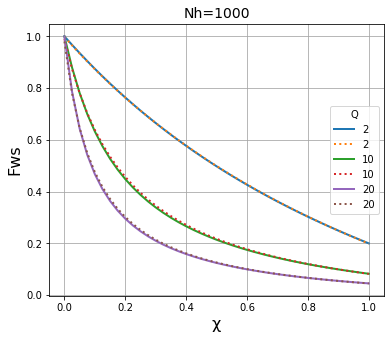
\includegraphics[width=7cm]{221115_fws_compare_1000.png}
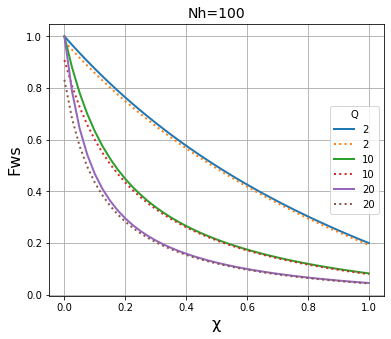
\includegraphics[width=7cm]{221115_fws_compare_100.png}
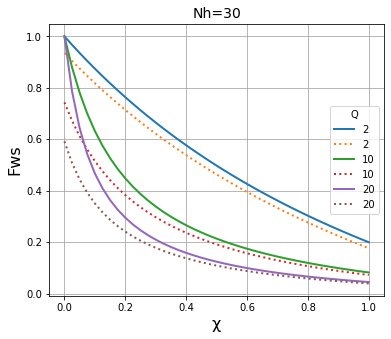
\includegraphics[width=7cm]{221115_fws_compare_30.png}
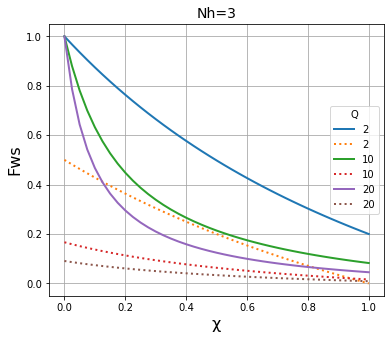
\includegraphics[width=7cm]{221115_fws_compare_3.png}
\caption{\textbf{The inbreeding coefficient $F_{WS}$ is inversely related to $\chi$.}  Colours represent different values of $Q$.  Solid lines show the results obtained from equation \ref{eq:supp_hwhs} and dotted lines show the results obtained by Markov chain simulation of coalescence times.  When $N_h$ is above 100 (top panels) the two methods give very similar results.  When $N_h = 30$ (bottom left panel) equation \ref{eq:supp_hwhs} tends to overestimate $F_{WS}$ at low values of $\chi$ as compared with the results obtained by Markov chain simulation.  When $N_h = 3$ (bottom right panel) these differences are magnified and equation \ref{eq:supp_hwhs} is very unreliable. 
\href{https://github.com/d-kwiat/gtg/blob/main/fws_compare_methods.ipynb}{View code}
}
\label{fig:supp_fws_compare_methods}
\end{figure}

\subsection{Confounding of \texorpdfstring{$F_{WS}$}{Fws} by local population structure.}
\label{supp_fws_pop_structure}  

Estimates of $F_{WS}$ might be unreliable if there is a high degree of local population structure within the geographical area that we are sampling from, e.g. if we are sampling from a region with extremely mountainous or densely forested terrain, such that people and parasites rarely move between different villages.  If we let $H_R$ be the heterozygosity of the region that we are sampling from, and if $H_S$ is the heterozygosity of a single village, and $\widehat{H}_W$ the mean of within-host heterozygosity in a village, then 

\begin{equation*}
F_{WS} = \frac{F_{WR} - F_{SR}}{1 - F_{SR}}
\end{equation*}

where $F_{WR} = 1 - \widehat{H}_W / H_R$ and $F_{SR} = 1 - H_S / H_R$.  

If $F_{SR}$ is small, then $F_{WS} \approx F_{WR}$ so it does not matter if we aggregate samples between villages.  However if local subpopulations are highly differentiated from each other, i.e. if $F_{SR}$ is large, then it is essential to use samples from a specific village when estimating $F_{WS}$ because aggregating samples from different villages could cause a substantial overestimate.

This might explain the surprising observation that $F_{WS}$ appears to be close to 1 in regions of Papua New Guinea where \textit{P. falciparum} infection is at a very high prevalence \cite{Manske2012,MalariaGEN2021}.  This could be due to confounding by local population structure, since these are mountainous jungle regions where the human population is divided into many small isolated communities, which might cause local parasite subpopulations to become highly differentiated from each other.

\end{document}